\subsection{Probability Models for Measurement Data}

\todo{Chapter 1}

\subsubsection{Random Variables}
		{
			% Extra row height for fractions and integrals
			\setlength{\extrarowheight}{3pt}
		
			\begin{twoColTable}
				\hline
				\twoColHdrRow{Random Variables}\\
				\hline
				\textbf{Definition}
					& $X:\Omega \longrightarrow W\textsubscript{x}$\\
				\hline	
				\textbf{Example}
					& A Coin is thrown three times, head and tails is observed:\\
					& $\Omega = \left\{hhh, hht, htt, hth, ttt, tth, thh, tht\right\}$\\
					& Total number of heads $W\textsubscript{x}=\left\{0,1,2,3\right\}$\\
					& Total number of tails $W\textsubscript{x}=\left\{0,1,2,3\right\}$\\
					& Number of heads minus tails $W\textsubscript{x}=\left\{-3,-1,1,3\right\}$\\
				\hline
				\hline
				\twoColHdrRow{Probability Mass Function}\\
				\hline
				\textbf{Definition}
					& The probability function of a discrete random variable:\\
					&$P(X = x)$\\
				\hline	
				\textbf{Example}
				&
				\begin{tabular}{l|l*{4}{c}r}
					x & 0 & 1 & 2 & 3 \\
					\hline
					$P(X = x)$ & $\frac{1}{8}$ & $\frac{3}{8}$ & $\frac{3}{8}$ & $\frac{1}{8}$\\
				\end{tabular}\\
				\hline	
			\end{twoColTable}
		}

	\subsubsection{Probability Distributions}
		{
			% Extra row height for fractions and integrals
			\setlength{\extrarowheight}{3pt}
		
			\begin{twoColTable}
				\hline
				\twoColHdrRow{Cumulative Density Function (cdf)}\\
				\hline
				\textbf{Definition}
					& $F(x) = P(X \leq x)$\\
				\hline	
				\textbf{Properties}
					& $P(a < X \leq b) = F(b) - F(a)$\\
					& $0 \leq F(x) \leq 1$\\
					& $P(X = a) = F(a) - F(a) = 0$\\
				\hline
			\end{twoColTable}
			\newpage
			\begin{twoColTable}
				\hline
				\twoColHdrRow{Probability Density Function (pdf)}\\
				\hline
				\textbf{Definition}
					& $ f(x) = \diff{F(x)}{x}$\\[1ex] % bottom padding for fraction
				\hline	
				\textbf{Properties}
					& $f(x) \geq 0$\\[1ex] % bottom padding for integral
					& $ P(a < X \leq b) = F(b) - F(a) = \int\limits_a^b f(x)\mathrm{d}x$\\[1ex] % bottom padding for integral
					& $\int\limits_{-\infty}^{\infty} f(x)\mathrm{d}x = 1$\\[1ex] % bottom padding for integral
				\hline
			\end{twoColTable}
		}
		
		\begin{figure}[H]\centering
			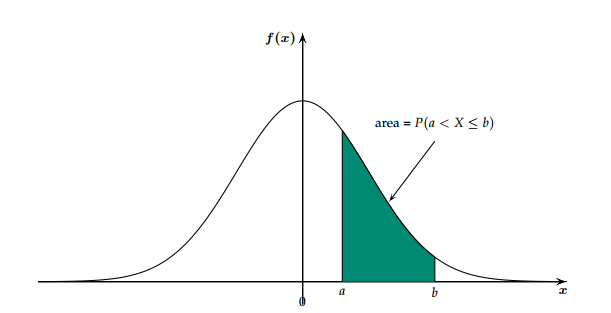
\includegraphics[scale=1]{images/ProbabilityDensityRV.png}
			\caption{Probability density of a random variable and the probability of measuring a value from (a,b]}
		\end{figure}
	
	\subsubsection{Summary Statistics of Continuous Distributions}
		{
			% Extra row height for fractions and integrals
			\setlength{\extrarowheight}{3pt}
			
			\begin{twoColTable}
				\hline
				\textbf{Expected value}
										& Discrete: $\mathrm{E}(X) = \sum\limits_{i} x_i P(X = x_i)$\\
										& Continuous: $\mathrm{E}(X) = \mu_X = \int\limits_{-\infty}^{\infty} x \cdot f(x) \mathrm{d}x$\\[1ex] % bottom padding for integral
				\hline
				\textbf{Variance}
					& $\mathrm{var}(X) = \sigma_x^2 = \mathrm{E}((X - \mathrm {E}(X))^2) =  \int\limits_{-\infty}^{\infty} (x - \mathrm{E}(X))^2 \cdot f(x) \mathrm{d}x$\\[1ex] % bottom padding for integral
				\hline
				\textbf{Quantile}
					& $P(X \leq q(\alpha)) = \alpha$\\
					& $F(q(\alpha)) = \alpha$\\
					& $q(\alpha) = F^{-1}(\alpha)$\\
					& {\color{red}Note: When you're asked for the $50\%$-quantile, that means $\alpha = 50\%$, and you must find $q(0.5)$}\\
				\hline
			\end{twoColTable}
		}
		
		\begin{figure}[H]\centering
			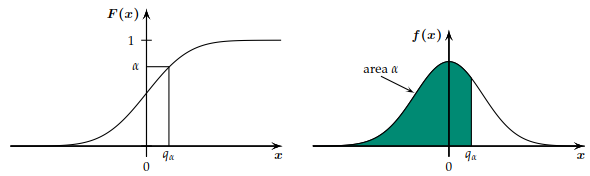
\includegraphics[scale=1]{images/quantile.png}
			\caption{Quantiles}
		\end{figure}
		
		\subsubsection{Important Distributions}
			\paragraph{Uniform Distribution}
				\RTheory%
				{%
					$$\begin{aligned}[t]
						f(x) 			&= 	\begin{cases}
												\frac{1}{b - a} 	& a \leq x \leq b\\
												0					& \mathrm{otherwise}\\ 
											\end{cases}\\
						F(x) 			&= 	\begin{cases}
												0					& x < a\\
												\frac{x-a}{b - a} 	& a \leq x \leq b\\
												1					& x > b\\ 
											\end{cases}\\
						\mathrm{E}(x) 	&= \frac{a+b}{2}\\
						\mathrm{var}(x) &= \frac{(b-a)^2}{12}\\
					\end{aligned}$$
				}{sections/ProbabilityStatistics/ProbabilityModels/ImportantDistributions/uniformTheory.R}
				
				\paragraph{Exponential Distribution}
				\RTheory%
				{%
					$$\begin{aligned}[t]
						f(x) 			&= 	\begin{cases}
												\lambda\cdot e^{-\lambda\cdot x} 	& x \geq 0\\
												0					& \mathrm{otherwise}\\ 
											\end{cases}\\
						F(x) 			&= 	\begin{cases}
												1- \lambda\cdot e^{-\lambda\cdot x} 	& x \geq 0\\
												0					& \mathrm{otherwise}\\ 
											\end{cases}\\
						\mathrm{E}(x) 	&= \frac{1}{\lambda}\\
						\mathrm{var}(x) &= \frac{1}{\lambda^2}\\
					\end{aligned}$$
				}{sections/ProbabilityStatistics/ProbabilityModels/ImportantDistributions/exponentialTheory.R}